\subsection{Image classification}

Opti-CAM is evaluated quantitatively using classification metrics and qualitatively by visualizing saliency maps.

%------------------------------------------------------------------------------
%------------------------------------------------------------------------------
\begin{table}
\centering
\footnotesize
\setlength{\tabcolsep}{4pt}
\renewcommand{\arraystretch}{0.8}
\begin{tabular}{lrrrr|rrrr} \toprule
\mr{2}{\Th{Method}}                                & \mc{4}{\Th{ResNet50}} & \mc{4}{\Th{VGG16}} \\ \cmidrule{2-9}
                                                   & {$\AD\!\downarrow$} & {$\AG\!\uparrow$} & {$\AI\!\uparrow$} & \mc{1}{T} & {$\AD\!\downarrow$} & {$\AG\!\uparrow$} & {$\AI\!\uparrow$} & \mc{1}{T} \\ \midrule
Fake-CAM                &  0.8 &  1.6 & 46.0 &  0.00 &  0.5 &  0.6 & 42.6 &  0.00 \\ \midrule
Grad-CAM                & 12.2 & 17.6 & 44.4 &  0.03 & 14.2 & 14.7 & 40.6 &  0.02 \\
Grad-CAM++              & 12.9 & 16.0 & 42.1 &  0.03 & 17.1 & 10.2 & 33.4 &  0.02 \\
Score-CAM               &  8.6 & 26.6 & 56.7 & 15.22 & 13.5 & 15.6 & 41.7 &  3.11 \\
Ablation-CAM            & 12.5 & 16.4 & 42.8 & 18.26 & 15.5 & 12.6 & 36.9 &  2.98 \\
XGrad-CAM               & 12.2 & 17.6 & 44.4 &  0.03 & 13.8 & 14.8 & 41.2 &  0.02 \\
Layer-CAM               & 15.6 & 15.0 & 38.8 &  0.08 & 48.9 &  3.1 & 13.5 &  0.07 \\
ExPerturbation          & 38.1 &  9.5 & 22.5 & 152.96 & 43.0 &  7.1 & 20.5 & 83.20 \\
\hline
Opti-CAM                & \tb{ 1.5} & \tb{68.8} & \tb{92.8} &  4.15 &  \tb{1.3} & \tb{71.2} & \tb{92.7} & 3.94 \\
\bottomrule
\end{tabular}
\caption{\emph{Classification metrics} on ImageNet validation set, using CNNs. $\AD$/$\AI$: 
average drop/increase \autocite{chattopadhay2018grad}; $\AG$: average gain (ours); 
$\downarrow$ / $\uparrow$: lower / higher is better; 
T: \iavr{Average time (sec) per batch of 8 images. Bold: best, excluding Fake-CAM.}}
\label{tab:imagenet-cnn}
% \vspace{-0.2cm}
\end{table}
%------------------------------------------------------------------------------
% FakeCAM~\citep{poppi2021revisiting}
% Grad-CAM ~\citep{selvaraju2017grad}
% Grad-CAM++~\cite{chattopadhay2018grad}
% ScoreCAM~\citep{wang2020score} 
% AblationCAM~\citep{ramaswamy2020ablation}
% XGrad-CAM~\citep{fu2020axiom} 
% LayerCAM~\citep{jiang2021layercam} 
% ExPerturbation~\citep{fong2019understanding}
%\modify{HiRes-CAM} &\modify{12.2}&\modify{17.6}&\modify{44.4}&\modify{0.03}&\modify{15.8}&\modify{13.2}&\modify{37.8}&\modify{0.02}\\

%------------------------------------------------------------------------------


\paragraph{CNN}

\autoref{tab:imagenet-cnn} shows ImageNet classification metrics using \Th{VGG16} and \Th{ResNet50}. Our Opti-CAM brings impressive performance in terms of average drop ($\AD$) and Average Increase ($\AI$) metrics. That is, not only impressive improvement over baselines, but near-perfect: near-zero $\AD$ and above 90\% $\AI$. \redred{Our new metric $\AG$ is lower, around 70\% for Opti-CAM, but this is still several times higher than for all the other methods.}

Interestingly, Fake-CAM~\citep{poppi2021revisiting} is the winner in terms of $\AD$ and second or third best in $\AI$ after Opti-CAM and Score-CAM, but fails completely $\AG$. This is expected and makes Fake-CAM uninteresting as it should be: By only masking one pixel, the classification score can hardly drop (0.8\% on ResNet50) and while it increases very often (on 46\% of images), the gain is as little as the drop (0.7\%). This makes the pair ($\AD$, $\AG$) sufficient as primary metrics and $\AI$ can be thought of as secondary, if important at all.

In the supplementary material we report \emph{insertion} (I) and \emph{deletion} (D) metrics along with failure cases of Opti-CAM. The latter indicate that our saliency maps are not incorrect as a whole, but capturing more parts of the object, more instances or more background context results in larger or several disconnected salient regions. This does not let the classifier focus on a single discriminative region when pixels are processed sequentially by increasing saliency. Rather, I/D favor smaller and more compact saliency maps.


\autoref{tab:imagenet-cnn} also includes average execution time per image over the 1000-image ImageNet subset for all methods. Opti-CAM is slower than gradient-based methods that require only one pass through the network, but on par or faster than gradient-free methods. Indeed, we use a maximum of 100 iterations with one forward/backward pass per iteration, while Score-CAM and Ablation-CAM perform as many forward passes as channels. Hence they are much slower on ResNet50 than VGG16. ExtremalPerturbation does not depend on the number of channels but is very slow by performing a complex optimization in the image space.

%------------------------------------------------------------------------------
%------------------------------------------------------------------------------
\begin{table}
    \centering
    \footnotesize
    \setlength{\tabcolsep}{4pt}
    \renewcommand{\arraystretch}{0.8}
    \begin{tabular}{lrrrr|rrrr} \toprule
        \mr{2}{\Th{Method}}& \mc{4}{\Th{ViT-B}} & \mc{4}{\Th{DeiT-B}} \\ \cmidrule{2-9}
        & {$\AD\!\downarrow$} & {$\AG\!\uparrow$} & {$\AI\!\uparrow$} & \mc{1}{T} & {$\AD\!\downarrow$} & {$\AG\!\uparrow$} & {$\AI\!\uparrow$} & \mc{1}{T} \\ \midrule
        Fake-CAM            &  0.3 &  0.4 & 48.3 &  0.00 &  0.6 &  0.3 & 44.6 &  0.00 \\ \midrule
        Grad-CAM            & 69.4 &  2.5 & 12.4 &  0.14 & 33.5 &  1.7 & 12.5 &  0.11 \\
        Grad-CAM            & 86.3 &  1.5 &  1.0 &  0.15 & 50.7 &  0.9 &  7.2 &  0.13 \\
        Score-CAM           & 32.0 &  6.2 & 33.0 & 23.69 & 53.6 &  2.2 & 12.2 & 22.47 \\
        XGrad-CAM           & 88.1 &  0.4 &  4.3 &  0.13 & 80.5 &  0.3 &  4.1 &  0.12 \\
        Layer-CAM           & 82.0 &  0.2 &  2.9 &  0.24 & 88.9 &  0.4 &  2.6 & 0.24\\
        ExPerturbation      &28.8&6.2&24.4&133.52&60.9&2.0&8.5&129.12\\
        RawAtt              & 92.6 &  0.2 &  2.8 &  0.02 & 95.3 &  0.0 &  1.8 &  0.02 \\
        Rollout             & 42.1 &  5.6 & 20.9 &  0.02 & 55.2 &  0.8 &  7.9 &  0.02 \\
        TIBAV               & 81.7 &  0.8 &  5.8 &  0.16 & 62.3 &  0.7 &  7.1 &  0.16 \\\midrule
        Opti-CAM            & \tb{ 0.6} &   \tb{18.0} & \tb{90.1} &    16.05 & \tb{ 0.9} & \tb{26.0} & \tb{83.5} &    15.17 \\ \bottomrule
    \end{tabular}
    \caption{}
    %\caption{\emph{Classification metrics} on ImageNet validation set, using transformers. $\AD$/$\AI$: average drop/increase
    %\autocite{chattopadhay2018grad}; $\AG$: average gain (ours); $\downarrow$ / $\uparrow$: lower / higher is better. \iavr{T: Average time (sec) per batch of 8 images. Bold: best, excluding Fake-CAM.}}
    \label{tab:imagenet-trans}
\end{table}
%------------------------------------------------------------------------------
%Fake-CAM~\citep{poppi2021revisiting}    &  0.3 &  0.4 & 48.3 &  0.00 &  0.6 &  0.3 & 44.6 &  0.00 \\ \midrule
%Grad-CAM~\citep{selvaraju2017grad}      & 69.4 &  2.5 & 12.4 &  0.14 & 33.5 &  1.7 & 12.5 &  0.11 \\
%Grad-CAM++~\cite{chattopadhay2018grad}  & 86.3 &  1.5 &  1.0 &  0.15 & 50.7 &  0.9 &  7.2 &  0.13 \\
%Score-CAM~\citep{wang2020score}         & 32.0 &  6.2 & 33.0 & 23.69 & 53.6 &  2.2 & 12.2 & 22.47 \\
%XGrad-CAM~\citep{fu2020axiom}           & 88.1 &  0.4 &  4.3 &  0.13 & 80.5 &  0.3 &  4.1 &  0.12 \\
%Layer-CAM~\citep{jiang2021layercam}     & 82.0 &  0.2 &  2.9 &  0.24 & 88.9 &  0.4 &  2.6 & 0.24\\
%ExPerturbation~\citep{fong2019understanding}&28.8&6.2&24.4&133.52&60.9&2.0&8.5&129.12\\
%RawAtt~\citep{dosovitskiy2020image}     & 92.6 &  0.2 &  2.8 &  0.02 & 95.3 &  0.0 &  1.8 &  0.02 \\
%Rollout~\citep{abnar2020quantifying}    & 42.1 &  5.6 & 20.9 &  0.02 & 55.2 &  0.8 &  7.9 &  0.02 \\
%TIBAV~\cite{chefer2021transformer}      & 81.7 &  0.8 &  5.8 &  0.16 & 62.3 &  0.7 &  7.1 &  0.16 \\
%\modify{HiRes-CAM~\citep{draelos2020use}} &\modify{98.4}&\modify{0.0}&\modify{0.7}&\modify{0.03}&\modify{97.2}&\modify{0.0}&\modify{1.2}&\modify{0.03} \\
%\hline
%Opti-CAM (ours)                         & \tb{ 0.6} &   \tb{18.0} & \tb{90.1} &    16.05 & \tb{ 0.9} & \tb{26.0} & \tb{83.5} &    15.17 \\ \bottomrule
%------------------------------------------------------------------------------

\paragraph{Transformers}

\autoref{tab:imagenet-trans} shows ImageNet classification metrics using ViT \iavr{and DeiT}. Unlike CAM-based methods that rely on a class-specific linear combination of feature maps, raw attention~\citep{dosovitskiy2020image} and rollout~\citep{abnar2020quantifying} use the attention map of the [CLS] token from the last attention block and from all blocks respectively. \iavr{This attention map depends only on the particular image and not on the target class, hence it is not really comparable. TIBAV~\cite{chefer2021transformer} uses both instance-specific and class-specific information.

Opti-CAM outperforms all other methods dramatically, reaching near-zero $\AD$ and $\AI$ above 80 or 90\%. \redred{According to our new $\AG$ metric, Opti-CAM still works while all other methods fail, but $\AG$ is much more conservative than $\AI$. On ViT-B for example, the classification score increases for 90.1\% of the images by masking with Opti-CAM, but the gain is only 18.0\% on average.}}

%------------------------------------------------------------------------------
\begin{figure*}[t]
\newcommand{\sizeS}{.125}
\newcommand{\sizeP}{.125}
\newcommand{\hh}{.175\textwidth}
\newcommand{\ww}{.200\textwidth}
\setlength{\tabcolsep}{2pt}
\centering
\scriptsize
%\setlength{\tabcolsep}{2pt}
\begin{tabular}{cccccccc}
	& Input image &  Grad-CAM  & Grad-CAM++ & Score-CAM & Ablation-CAM & XGrad-CAM & Opti-CAM 
 \\

	\rotatebox{90}{~Grass Snake} &
	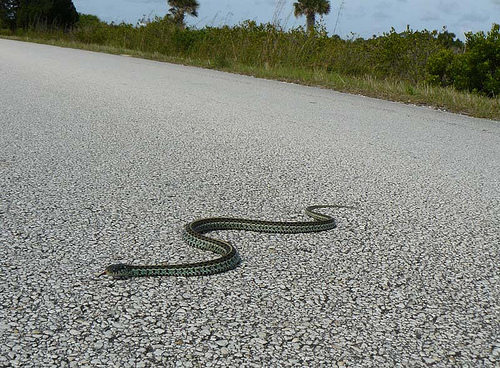
\includegraphics[trim={36mm 10mm 32mm 10mm},clip, width=\sizeP\textwidth]{fig/select/ILSVRC2012_val_00000006.JPEG}&
	\fig[\sizeS]{select/ILSVRC2012_val_00000006JPEG_vgg_GradCAM_vis.png} &
	\fig[\sizeS]{select/ILSVRC2012_val_00000006JPEG_vgg_GradCAMPlusPlus_vis.png} &
	\fig[\sizeS]{select/ILSVRC2012_val_00000006JPEG_vgg_ScoreCAM_vis.png} &
	\fig[\sizeS]{select/ILSVRC2012_val_00000006JPEG_vgg_AblationCAM_vis.png} &
	\fig[\sizeS]{select/ILSVRC2012_val_00000006JPEG_vgg_XGradCAM_vis.png} &
	\fig[\sizeS]{select/ILSVRC2012_val_00000006JPEG_vgg_versionP0_vis.png}  \\

	\rotatebox{90}{~Tricycle} &
	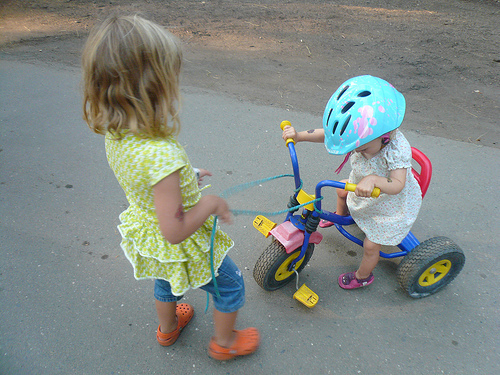
\includegraphics[trim={28mm 10mm 39mm 10mm},clip, width=\sizeP\textwidth]{fig/select/ILSVRC2012_val_00000069.JPEG}&
	\fig[\sizeS]{select/ILSVRC2012_val_00000069JPEG_vgg_GradCAM_vis.png} &
	\fig[\sizeS]{select/ILSVRC2012_val_00000069JPEG_vgg_GradCAMPlusPlus_vis.png} &
	\fig[\sizeS]{select/ILSVRC2012_val_00000069JPEG_vgg_ScoreCAM_vis.png} &
	\fig[\sizeS]{select/ILSVRC2012_val_00000069JPEG_vgg_AblationCAM_vis.png} &
	\fig[\sizeS]{select/ILSVRC2012_val_00000069JPEG_vgg_XGradCAM_vis.png} &
	\fig[\sizeS]{select/ILSVRC2012_val_00000069JPEG_vgg_versionP0_vis.png}  \\

	\rotatebox{90}{~Pneumonia} &
	\fig[\sizeS]{medical/chest_VGG16_GradCAM_1_img.png} &
	\fig[\sizeS]{medical/chest_VGG16_GradCAM_1_vis.png} &
	\fig[\sizeS]{medical/chest_VGG16_GradCAMPlusPlus_1_vis.png} &
	\fig[\sizeS]{medical/chest_VGG16_ScoreCAM_1_vis.png} &
	\fig[\sizeS]{medical/chest_VGG16_AblationCAM_1_vis.png} &
	\fig[\sizeS]{medical/chest_VGG16_XGradCAM_1_vis.png} &
	\fig[\sizeS]{medical/chest_VGG16_OptCAM_plain_1_vis.png}  \\


	\rotatebox{90}{~Pylorus} &
	\fig[\sizeS]{medical/kvasir_Resnet50_GradCAM_3_img.png} &
	\fig[\sizeS]{medical/kvasir_VGG16_GradCAM_3_vis.png} &
	\fig[\sizeS]{medical/kvasir_VGG16_GradCAMPlusPlus_3_vis.png} &
	\fig[\sizeS]{medical/kvasir_VGG16_ScoreCAM_3_vis.png} &
	\fig[\sizeS]{medical/kvasir_VGG16_AblationCAM_3_vis.png} &
	\fig[\sizeS]{medical/kvasir_VGG16_XGradCAM_3_vis.png} &
	\fig[\sizeS]{medical/kvasir_VGG16_OptCAM_plain_3_vis.png}  \\

\end{tabular}
\caption{Saliency maps obtained by different methods for ImageNet (top two rows), Chest X-ray (row 3) and Kvasir (row 4) with VGG. \iavr{Ground truth class shown on the left of the input image.}}
\label{fig:vis-in-chest-n-kvasir-resnet}
% \vspace{-0.4cm}
\end{figure*}
%------------------------------------------------------------------------------

\paragraph{Visualization}

\autoref{fig:vis-in-chest-n-kvasir-resnet} illustrates saliency map examples from ImageNet, Chest X-ray and Kvasir datasets. Opti-CAM saliency map is in general more spread out. This better highlights full objects, multiple instances or \iavr{background context, which may be taken into account by the model. On Chest X-ray, Opti-CAM and Score-CAM are the only methods that capture the chest, while all others focus on image corners.} More examples on datasets and networks \redred{as well as quantitative evaluation on medical data} are given in the supplementary material.
